\documentclass[a4paper]{article}

% bloc : évite un changement de page
% completemulti : ajoute une case : aucune bonne réponse
%\newcommand{\repRel}{../..}
%\input{\repRel/Style/packages}
%%\input{\repRel/Style/new_style}
%\input{\repRel/Style/macros_SII}
%%\input{\repRel/Style/environment}

\usepackage[francais,bloc,completemulti,ensemble]{automultiplechoice}
%\usepackage[francais,bloc,completemulti]{automultiplechoice} 
\usepackage{amsmath}
% ensemble : feuille de questions et feuille de réponse séparées

\usepackage{multicol}

%% Pour le python %%
\usepackage{listingsutf8}

\lstset{language=Python,
  inputencoding=utf8/latin1,
  breaklines=true,
  basicstyle=\ttfamily\small,
  keywordstyle=\bfseries\color{green!40!black},
  commentstyle=\itshape\color{purple!40!black},
  identifierstyle=\color{blue},
  stringstyle=\color{orange},
  upquote = true,
  columns=fullflexible,
  backgroundcolor=\color{gray!10},frame=leftline,rulecolor=\color{gray}}  
  
\definecolor{mygreen}{rgb}{0,0.6,0}

\lstset{
     literate=%
         {é}{{\'e}}1    
         {è}{{\`e}}1    
         {ê}{{\^e}}1    
         {à}{{\`a}}1
         {â}{{\^a}}1		 
         {ô}{{\^o}}1    
         {ù}{{\`u}}1    
         {î}{{\^i}}1    
}
\lstset{inputpath=code}

\usepackage{siunitx}
%\usepackage[utf8x]{inputenc}
%\usepackage[T1]{fontenc}

\begin{document}
%\AMCrandomseed{1233893}
%\setdefaultgroupmode{withoutreplacement} % Mélange des questions groupées

\graphicspath{{../Banque_SI/02_FTBO/images/}}
\element{ftbo}{
\begin{question}{ftbo 01}
Soit le schéma blocs suivant. Donner le FTBO.
\begin{center}
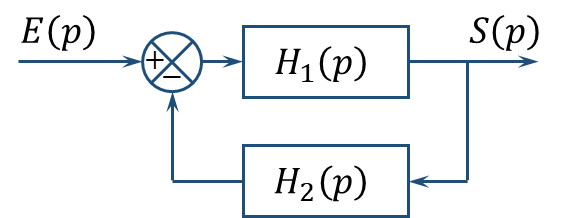
\includegraphics[width=6cm]{fig_01}
\end{center}

	\begin{reponses}	
	\bonne{$\text{FTBO}(p)=H_1(p)H_2(p)$}
	\mauvaise{$\text{FTBO}(p)=H_1(p)$}
	\mauvaise{$\text{FTBO}(p)=\dfrac{H_1(p)}{H_2(p)}$}
	\mauvaise{$\text{FTBO}(p)=\dfrac{H_1(p)}{1+H_1(p)H_2(p)}$}
	\mauvaise{$\text{FTBO}(p)=\dfrac{H_1(p)}{1-H_1(p)H_2(p)}$}
	\end{reponses}

\end{question}\\
}

\element{ftbo}{
\begin{question}{ftbo 02}
Soit le schéma blocs suivant. Donner le FTBO.
\begin{center}
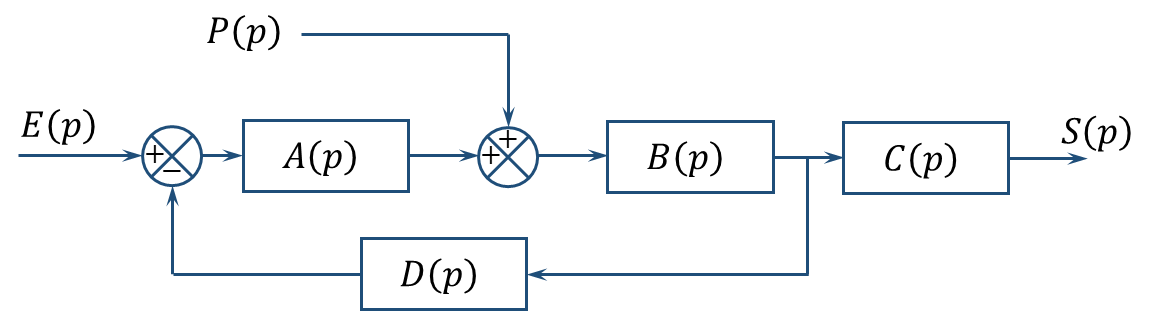
\includegraphics[width=8cm]{fig_02}
\end{center}

	\begin{reponses}	
	\bonne{$\text{FTBO}(p)=A(p)B(p)D(p)$}
	\mauvaise{$\text{FTBO}(p)=A(p)$}
	\mauvaise{$\text{FTBO}(p)=A(p)B(p)C(p)$}
	\mauvaise{$\text{FTBO}(p)=A(p)B(p)C(p)D(p)$}
	\mauvaise{$\text{FTBO}(p)=\dfrac{A(p)B(p)}{1+A(p)B(p)D(p)}$}
	\end{reponses}

\end{question}\\
}


%\element{ftbo}{
%\begin{question}{ftbo 03}
%Soit le schéma blocs suivant. Donner le FTBO.
%\begin{center}
%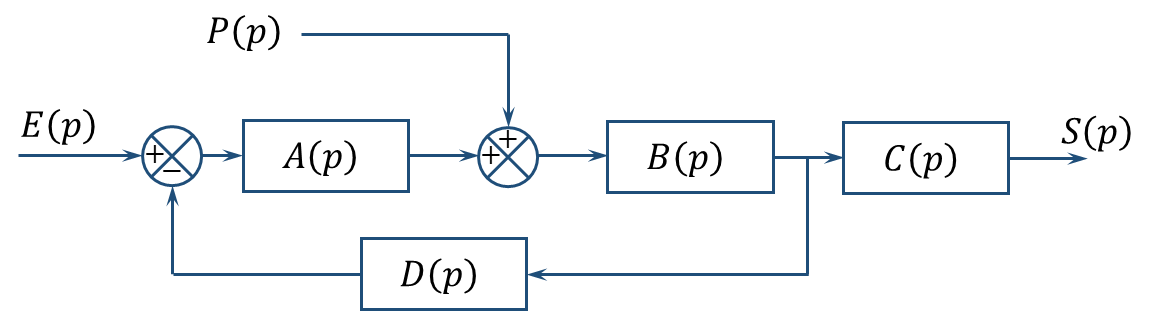
\includegraphics[width=6cm]{fig_03}
%\end{center}
%
%	\begin{reponses}	
%	\bonne{$\text{FTBO}(p)=$}
%	\mauvaise{$\text{FTBO}(p)=$}
%	\mauvaise{$\text{FTBO}(p)=$}
%	\mauvaise{$\text{FTBO}(p)=$}
%	\mauvaise{$\text{FTBO}(p)=$}
%	\end{reponses}
%
%\end{question}\\
%}


\element{ftbo}{
\begin{question}{ftbo 04}
Soit le schéma blocs suivant. Donner le FTBO.
\begin{center}
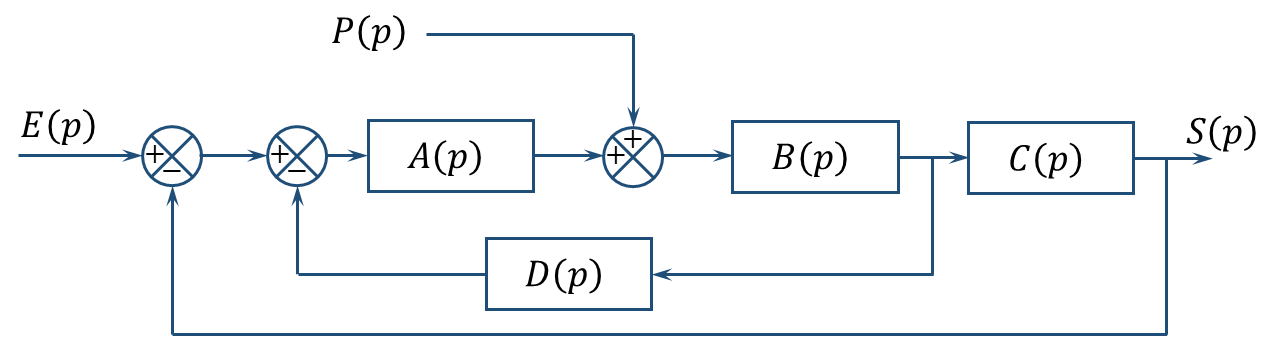
\includegraphics[width=8cm]{fig_04}
\end{center}

	\begin{reponses}	
	\bonne{$\text{FTBO}(p)=\dfrac{A(p)B(p)C(p)}{1+A(p)B(p)D(p)}$}
	\mauvaise{$\text{FTBO}(p)=A(p)B(p)$}
	\mauvaise{$\text{FTBO}(p)=A(p)B(p)C(p)D(p)$}
	\mauvaise{$\text{FTBO}(p)=A(p)B(p)C(p)$}
	\mauvaise{$\text{FTBO}(p)=B(p)C(p)$}
	\end{reponses}

\end{question}\\
}


\element{ftbo}{
\begin{question}{ftbo 05}
Soit le schéma blocs suivant. Donner le FTBO.
\begin{center}
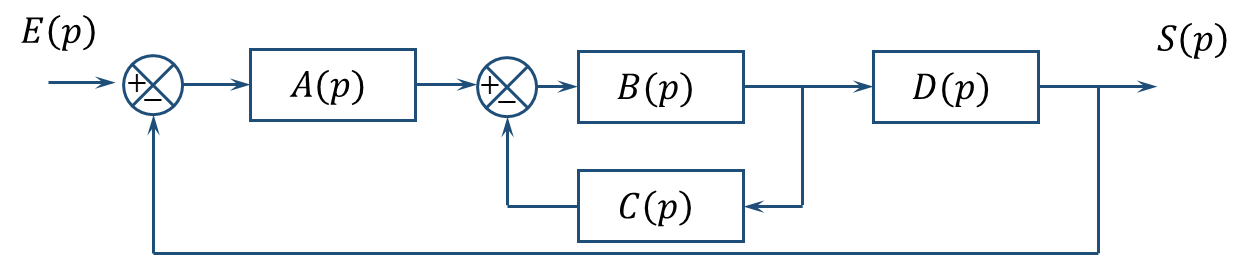
\includegraphics[width=8cm]{fig_05}
\end{center}

	\begin{reponses}	
	\bonne{$\text{FTBO}(p)=\dfrac{A(p)B(p)D(p)}{1+B(p)C(p)}$}
	\mauvaise{$\text{FTBO}(p)=A(p)B(p)C(p)D(p)$}
	\mauvaise{$\text{FTBO}(p)=A(p)B(p)C(p)$}
	\mauvaise{$\text{FTBO}(p)=B(p)C(p)$}
	\mauvaise{$\text{FTBO}(p)=A(p)B(p)D(p)$}
	\end{reponses}

\end{question}\\
}


\element{ftbo}{
\begin{question}{ftbo 06}
Soit le schéma blocs suivant. Donner le FTBO.
\begin{center}
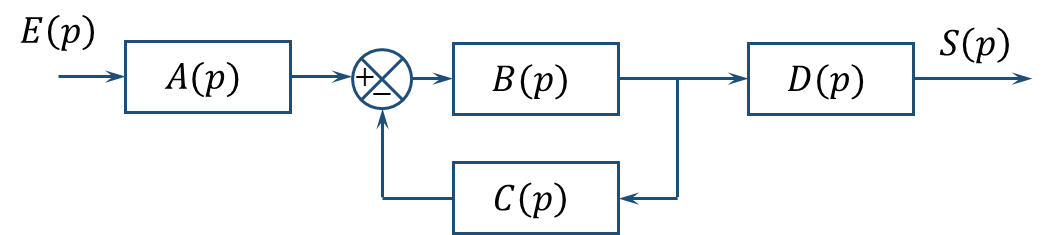
\includegraphics[width=8cm]{fig_06}
\end{center}

	\begin{reponses}	
	\bonne{$\text{FTBO}(p)=B(p)C(p)$}
	\mauvaise{$\text{FTBO}(p)=A(p)B(p)C(p)$}
	\mauvaise{$\text{FTBO}(p)=A(p)B(p)C(p)D(p)$}
	\mauvaise{$\text{FTBO}(p)=\dfrac{A(p)B(p)D(p)}{1+B(p)C(p)}$}
	\mauvaise{$\text{FTBO}(p)=A(p)B(p)D(p)$}
	\end{reponses}

\end{question}\\
}


\element{ftbo}{
\begin{question}{ftbo 07}
Soit le schéma blocs suivant. Donner le FTBO.

\begin{center}
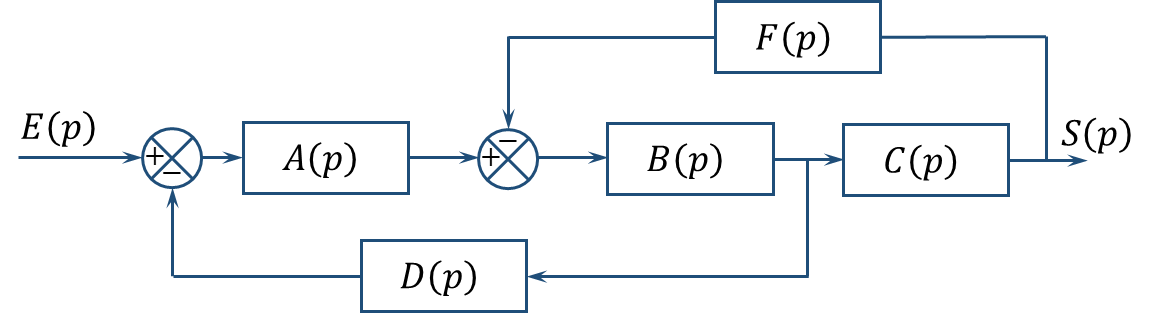
\includegraphics[width=8cm]{fig_07}
\end{center}

	\begin{reponses}	
	\bonne{$\text{FTBO}(p)=\dfrac{A(p)B(p)D(p)}{1+B(p)C(p)D(p)}$}
	\mauvaise{$\text{FTBO}(p)=A(p)B(p)D(p)$}
	\mauvaise{$\text{FTBO}(p)=A(p)B(p)C(p)D(p)$}
	\mauvaise{$\text{FTBO}(p)=\dfrac{A(p)B(p)C(p)}{1+A(p)B(p)D(p)}$}
	\mauvaise{$\text{FTBO}(p)=\dfrac{A(p)B(p)C(p)}{1+B(p)C(p)F(p)}$}
	\end{reponses}

\end{question}\\
}


\element{ftbo}{
\begin{question}{ftbo 08}
Soit le schéma blocs suivant. Donner le FTBO.
\begin{center}
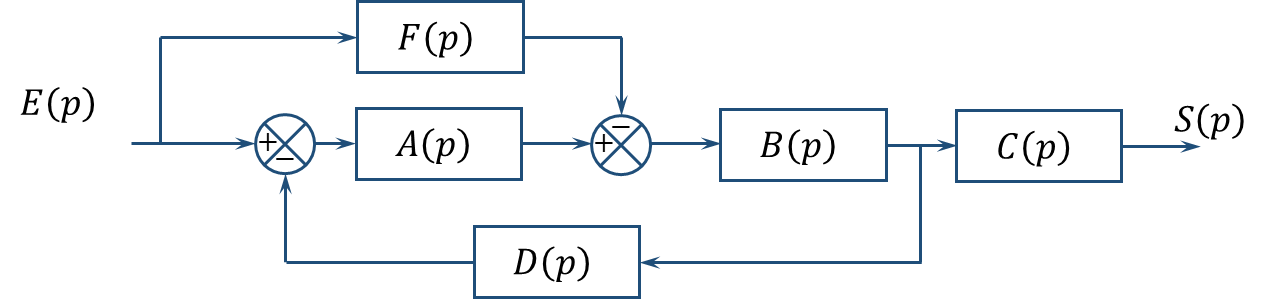
\includegraphics[width=8cm]{fig_08}
\end{center}

	\begin{reponses}	
	\bonne{$\text{FTBO}(p)=B(p)D(p)\dfrac{A(p)-F(p)}{1+B(p)D(p)F(p)}$}
	\mauvaise{$\text{FTBO}(p)=A(p)B(p)D(p)$}
	\mauvaise{$\text{FTBO}(p)=B(p)C(p)$}
	\mauvaise{$\text{FTBO}(p)=A(p)B(p)C(p)$}
	\mauvaise{$\text{FTBO}(p)=\dfrac{A(p)B(p)C(p)}{1+A(p)B(p)D(p)}$}
	\end{reponses}

\end{question}\\
}


\element{ftbo}{
\begin{question}{ftbo 09}
Soit le schéma blocs suivant. Donner le FTBO.
\begin{center}
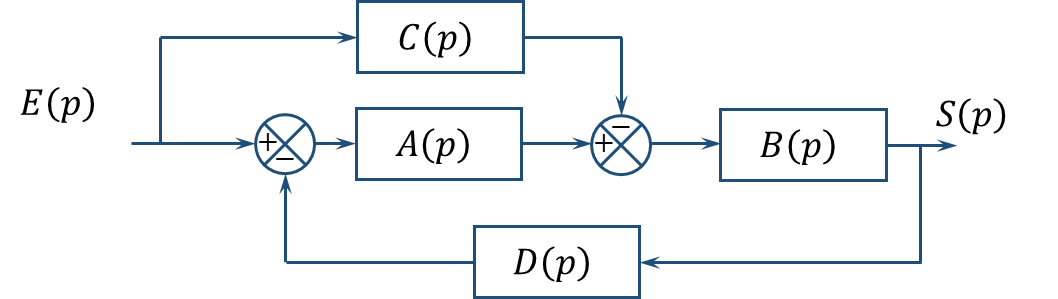
\includegraphics[width=8cm]{fig_09}
\end{center}

	\begin{reponses}	
	\bonne{$\text{FTBO}(p)=B(p)D(p)\dfrac{A(p)-C(p)}{1+B(p)D(p)C(p)}$}
	\mauvaise{$\text{FTBO}(p)=A(p)B(p)D(p)$}
	\mauvaise{$\text{FTBO}(p)=\left(A(p)-C(p)\right)B(p)D(p)$}
	\mauvaise{$\text{FTBO}(p)=A(p)B(p)C(p)$}
	\mauvaise{$\text{FTBO}(p)=\dfrac{A(p)-C(p)}{1+A(p)B(p)D(p)}$}
	\end{reponses}

\end{question}\\
}







\exemplaire{1}{
% Entetes sujet
\noindent{\bf QCM -- Codeurs incrémentaux}

\vspace*{.5cm}
% Questions
\restituegroupe{ftbo}

\AMCcleardoublepage


\AMCdebutFormulaire
% ENtetes
%{\large\bf Feuille de réponses :}
%
%\vspace{.5cm}
%
%\begin{minipage}[c]{.45\linewidth}
%\AMCcodeGridInt[h]{etu}{2}
%\end{minipage}
%\hfill
%\begin{minipage}[c]{.45\linewidth}
%\champnom{\fbox{
%\begin{minipage}{.9\linewidth}
%Nom et prénom :
%\vspace*{.5cm}\dotfill
%\vspace*{.5cm}\dotfill
%\vspace*{1mm}
%\end{minipage}
%}}
%\end{minipage}
%
%%%%%%%%
%
%
%
%\formulaire

% 
}

\end{document}